\documentclass[10pt]{article}

\usepackage[T1]{fontenc}
\usepackage{geometry}
\usepackage{amsmath, amssymb, amsthm}
\usepackage{yhmath}
\usepackage{graphicx}
\usepackage{caption}
\usepackage{subcaption}
\usepackage{xcolor}
\usepackage{float}
\usepackage{bm}
\usepackage{hyperref}

\geometry{a4paper, margin=1in}

\renewcommand{\labelenumi}{(\alph{enumi})}
\renewcommand{\vec}{\bm}
\DeclareMathOperator*{\argmax}{arg\,max}
\DeclareMathOperator*{\argmin}{arg\,min}
\DeclareMathOperator*{\trace}{trace}
\DeclareMathOperator*{\var}{var}

\newcommand{\C}{\mathbb{C}}
\newcommand{\R}{\mathbb{R}}
\newcommand{\Q}{\mathbb{Q}}
\newcommand{\Z}{\mathbb{Z}}
\newcommand{\N}{\mathbb{N}}

\setlength{\parindent}{0em}

\title{Nonparametric Regression}
\author{Satvik Saha}
\date{}

\begin{document}
    \noindent\textbf{IISER Kolkata} \hfill \textbf{Final Assignment}
    \vspace{3pt}
    \hrule
    \vspace{3pt}
    \begin{center}
    \LARGE{\textbf{MA5121: Nonparametric Statistics}}
    \end{center}
    \vspace{3pt}
    \hrule
    \vspace{3pt}
    Satvik Saha, \texttt{19MS154} \hfill \today
    \vspace{20pt}

    \setlength{\parskip}{1em}


    \paragraph{Problem 1} Consider the following samples. \begin{align*}
        X &: 35, 66, 58, 83, 71. \\
        Y &: 46, 56, 60, 49.
    \end{align*} The two-sided Mood test of scale gives a $p$-value of
    $0.2072$, and the two-sided Ansari-Bradley test gives a $p$-value of
    $0.5238$. Thus, we fail to reject the null hypothesis that $X$ and $Y$
    differ in variability at an $\alpha = 0.05$ level of significance.

    Given the sparsity of the data, it is difficult to give a definitive
    answer, especially since the visualization below seems to indicate that
    $X$ has greater variability than $Y$. A two-sided $F$-test for comparing
    variance (assuming that the distributions of $X$ and $Y$ are normal) gives
    a $p$-value of $0.1225$, and a 95\% confidence interval of $(0.52, 78)$
    for the ratio of variances.


    \begin{figure}[H]
        \centering
        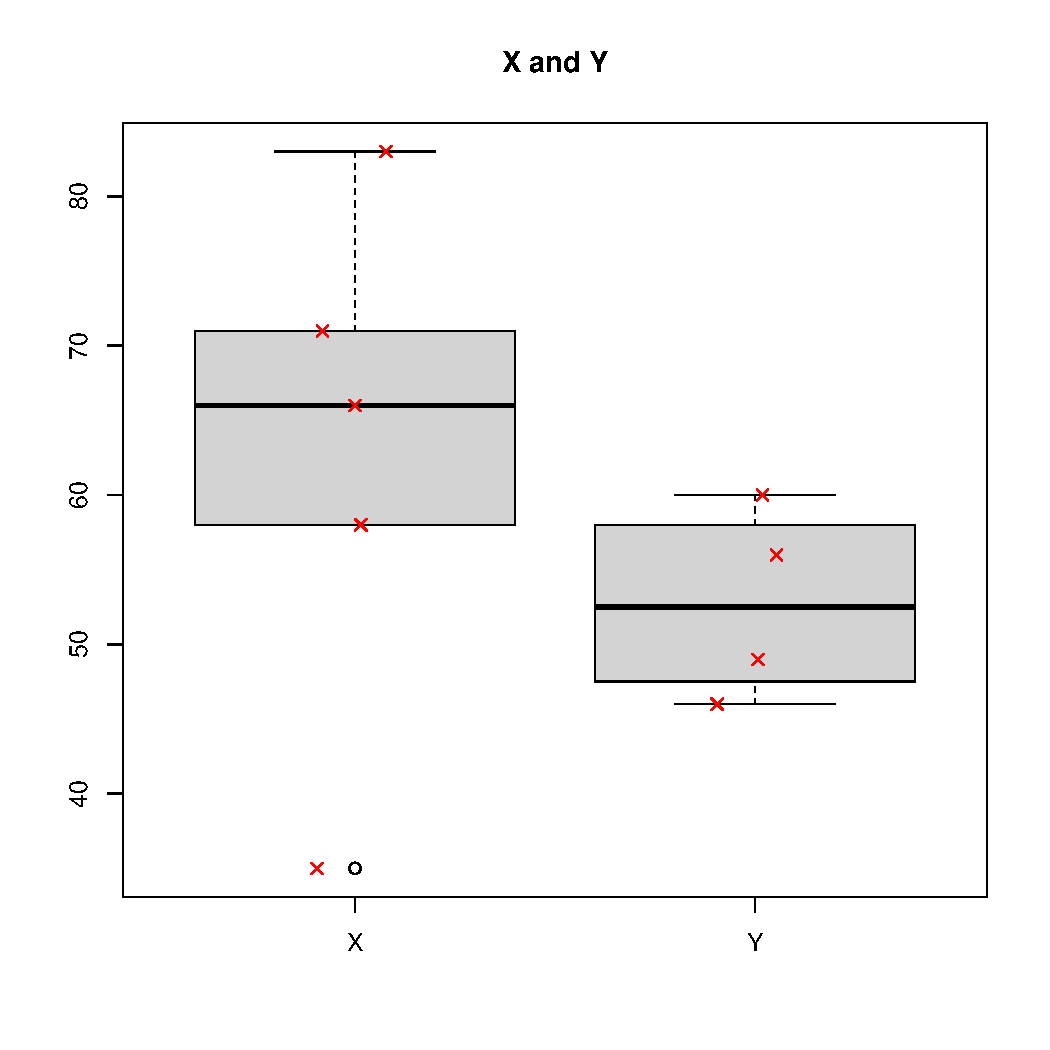
\includegraphics[width=0.8\textwidth, page = 1]{final_plots.pdf}
        \vspace{-2em}
        \caption{$X$ and $Y$.}
        \label{fig:scale_test}
    \end{figure}


    \clearpage

    \paragraph{Problem 2} Consider the following distributions of number of
    days until death (by tuberculosis infection) for mice. \begin{align*}
        \text{(Control) } A &: 5, 6, 7, 7, 8, 8, 8, 9, 12. \\
        \text{(Treated by drug) } B &: 7, 8, 8, 8, 9, 9, 12, 13, 14, 17.
    \end{align*} We set up the null hypothesis that the distributions of $A$
    and $B$ are identical, versus the alternative hypothesis that $A
    \stackrel{st}{<} B$.

    The Wilcoxon rank-sum test gives a $p$-value of around $0.02$, using which
    we reject the null hypothesis at a $0.05$ level of significance. Thus, we
    infer that the drug treatment has the positive effect of prolonging the
    number of days till death by tuberculosis infection for mice.

    We employ the one-sided Wilcoxon rank-sum test since we wish to determine
    whether the distributions of number of days (for the groups $A$ and $B$)
    are identical or not. We also discard the possibility that $A
    \stackrel{st}{>} B$. However, it is difficult to justify the assumption
    that the underlying distributions are continuous since our data is quite
    discrete, and thus the large number of ties may make the rank-sum test
    unreliable.

    The $t$-test for location, assuming normality (which can be justified to
    some extent via the Shapiro-Wilk test; the $t$-test is also quite robust
    to non-normality), also yields a $p$-value of around $0.022$, with which
    we may again reject the null hypothesis.

    \begin{figure}[H]
        \centering
        \includegraphics[width=0.8\textwidth, page = 2]{final_plots.pdf}
        \vspace{-2em}
        \caption{Days till death by tuberculosis for mice.}
        \label{fig:tuberculosis_treatment}
    \end{figure}

\end{document}
